\documentclass[a4paper, pdftex, english, 11pt]{article}

\usepackage[utf8]{inputenc}
\usepackage[T1]{fontenc}
\usepackage[english]{babel}
\usepackage[iso]{umlaute}
\usepackage{graphicx}
\usepackage{float}

\begin{document}
\section{Why is the penguin called \emph{"penguin"?}}
\subsection{Explanation 1}
The name originates from the Welsh word \emph{"Pen Gwyn"} (spoken like the english penguin). It means \emph{"white head"}. Sailors from \textbf{Wales} are said to have spotted and named them for the first time. (see also picture \ref{img:pen}).

\begin{figure}[H]
\begin{center}
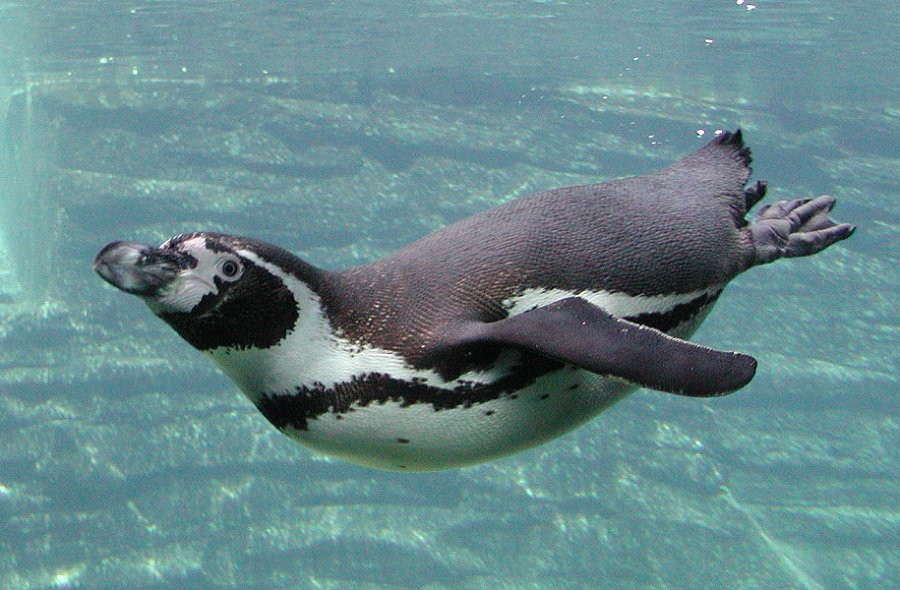
\includegraphics[width=4cm]{bilder/swim-Ping.jpg}
\caption{A living penguin}
\label{img:pen}
\end{center}
\end{figure}

\subsection{Explanation 2}
It is also said that the word \emph{"penguin"} origianlly was a common name for the also flightless \textbf{great auk} of the northern hemisphere, that went extinct in 1844 (see picture \ref{img:auk}).

\begin{figure}[H]
\begin{center}
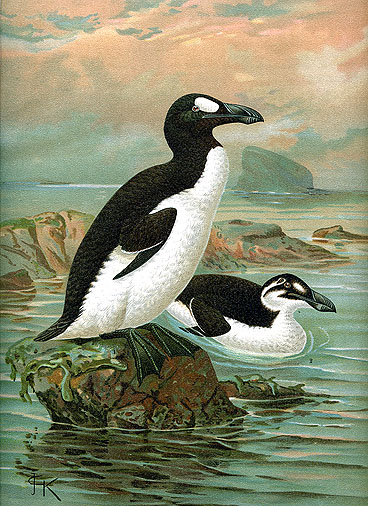
\includegraphics[width=5cm]{bilder/GreatAuk.jpg}
\caption{Great auks}
\label{img:auk}
\end{center}
\end{figure}

\newpage
\subsection{Explanation 3}
Another theory is that the name stems from the latin word \emph{"penguis"}. It means \emph{"fat"}. For sailors, fat was very important and it could be won from \textbf{penguins} (see picture \ref{img:tux}).

\begin{figure}[H]
\begin{center}

\includegraphics[width=5cm]{bilder/tux.png}
\caption{Tiny Tux}
\label{img:tux}
\end{center}
\end{figure}
\end{document}